% This text is Free and open Open Source.
% It's a part of presentation made by myself.
% It may be used only for academic purpose
% May, 2012
% Author: Seshagiri Prabhu
% Amrita Vishwa Vidyapeethm 
% seshagiriprabhu@gmail.com
% www.seshagiriprabhu.wordpress.com

\documentclass[12pt]{beamer}
\usetheme{Oxygen}
\usepackage{thumbpdf}
\usepackage{wasysym}
\usepackage{ucs}
\usepackage[utf8]{inputenc}
\usepackage{pgf,pgfarrows,pgfnodes,pgfautomata,pgfheaps,pgfshade}
\usepackage{verbatim}
\usepackage{listings}
\usepackage{courier}
\usepackage{caption}
\usepackage{verbatim} 
\usepackage{upquote}
\usepackage{graphics}
\usepackage{latexsym}
\usepackage{fixltx2e}
\usepackage{graphicx}
\usepackage{hyperref}
\usepackage{amssymb}
\usepackage{ragged2e}
\usepackage{amsmath}
\usepackage{mathtools}
\usepackage{framed,lipsum}
\usepackage{pgf}
\usepackage{fmtcount}% http://ctan.org/pkg/fmtcount
\usepackage{algorithm, algpseudocode}
\usepackage{caption}
\captionsetup[algorithm]{font=scriptsize}
\usepackage{etoolbox}
\usepackage{xcolor}
\makeatother
\newcommand\Colorhref[3][cyan]{\href{#2}{\small\color{#1}#3}}
\newcommand\Fontvi{\fontsize{5}{6}\selectfont}
%\renewcommand\tinyv{\@setfontsize\tinyv{4pt}{6}}
%\renewcommand\tiny{\@setfontsize\tiny{4pt}{6}}
\usepackage{xcolor}
\setbeamertemplate{itemize items}[default]
\setbeamertemplate{enumerate items}[default]
\def\SPSB#1#2{\rlap{\textsuperscript{\textcolor{red}{#1}}}\SB{#2}}
\def\SP#1{\textsuperscript{\textcolor{red}{#1}}}
\def\SB#1{\textsubscript{\textcolor{blue}{#1}}}

\usepackage{tikz}
\usetikzlibrary{decorations}
\usepackage{textcomp} 
\usetikzlibrary{snakes}
\usepackage{ifthen}
\usepackage[firstyear=2008,lastyear=2011]{moderntimeline}
\colorlet{color0}{blue}
\colorlet{color1}{olive}

\newcommand*{\hintfont}{}
\newcommand*{\hintstyle}[1]{{\hintfont\textcolor{color0}{#1}}}
\newcommand*{\listitemsymbol}{a~}
\newcommand*{\cventry}[7][.25em]{%
  \cvitem[#1]{#2}{%
    {\bfseries\raggedright #3}%
    \ifthenelse{\equal{#4}{}}{}{, \raggedright{\slshape#4}}%
    \ifthenelse{\equal{#5}{}}{}{,  \raggedright#5}%
    \ifthenelse{\equal{#6}{}}{}{, \raggedright#6}%
    .\strut%
    \ifx&#7&%
      \else{\newline{}\begin{minipage}[t]{\linewidth}\small\raggedright#7\end{minipage}}\fi}}
\newcommand*{\cvitem}[3][.25em]{%
  \begin{tabular}{@{}p{\hintscolumnwidth}@{\hspace{\separatorcolumnwidth}}p{\maincolumnwidth}@{}}%
      \raggedleft\hintstyle{#2} & {#3}%
  \end{tabular}%
  \par\addvspace{#1}}
\tlmaxdates{2008}{2011}
\newlength{\quotewidth}
\newlength{\hintscolumnwidth}
\setlength{\hintscolumnwidth}{0.175\textwidth}
\newlength{\separatorcolumnwidth}
\setlength{\separatorcolumnwidth}{0.025\textwidth}
\newlength{\maincolumnwidth}
\newlength{\doubleitemmaincolumnwidth}
\newlength{\listitemsymbolwidth}
\settowidth{\listitemsymbolwidth}{\listitemsymbol}
\newlength{\listitemmaincolumnwidth}
\newlength{\listdoubleitemmaincolumnwidth}
\setlength{\maincolumnwidth}{\dimexpr0.9\linewidth-\separatorcolumnwidth-\hintscolumnwidth\relax}
\makeatother

\newenvironment{variableblock}[3]{%
  \setbeamercolor{block body}{#2}
  \setbeamercolor{block title}{#3}
  \begin{block}{#1}}{\end{block}}

\usepackage{listings}
\usepackage{color}

\definecolor{mygreen}{rgb}{0,0.6,0}
\definecolor{mygray}{rgb}{0.5,0.5,0.5}
\definecolor{mymauve}{rgb}{0.58,0,0.82}
\lstset{
 breaklines=true, commentstyle=\color{mygreen}, stepnumber=1, tabsize=2, stringstyle=\color{mymauve}, numberstyle=\tiny\color{mygray}, rulecolor=\color{black}, morekeywords={make,mkdir,gcc, all, clean, F, OO}, basicstyle=\tiny\ttfamily,keywordstyle=\color{blue}, emph={CC, CFLAG, EXECS, PROG, OBJS, OBJECTS, PHONY}, emphstyle=\color{red}, emph={[2]\#using,\#define,\#ifdef,\#endif}, emphstyle={[2]\color{blue}}, stringstyle=\color{red}
}
\pdfinfo
{
  /Title       (SN 707 Software Protection)
  /Creator     (Seshagiri Prabhu N)
  /Author      (TeX)
}
\title{SN 707 Software Protection}
\subtitle{Assignment 2}
\author{Seshagiri Prabhu N}
\institute[Amrita Vishwa Vidyapeetham] % (optional)
{
  \begin{center}
    \tiny \textbf{AM.EN.P2CSN12028} \\ 
    M.Tech, Cyber Security and Networks\\
  	Amrita School of Engineering,
	Amritapuri Campus
  \end{center}  
}

\begin{document}
\frame{\titlepage}


\begin{frame}
  \frametitle{Outline}
  \tableofcontents[section=1,hidesubsections]
\end{frame}

\newcommand{\icon}[1]{\pgfimage[height=1em]{#1}}

%%%%%%%%%%%%%%%%%%%%%%%%%%%%%%%%%%%%%%%%%
%%%%%%%%%% Content starts here %%%%%%%%%%
%%%%%%%%%%%%%%%%%%%%%%%%%%%%%%%%%%%%%%%%%

\section{Invention}
\begin{frame}
	\frametitle{Invention}
	\begin{variableblock}{}{bg=orange,fg=black}{bg=green,fg=red}
		\begin{center}
			\vskip5mm
  			{\large AVAZ for autism}
  			\vskip5mm
  			\vskip5mm  			
		\end{center}
	\end{variableblock}
\end{frame}


\section{Inventor}
\begin{frame}
	\frametitle{Inventor: Invention Labs}
	\begin{center}
		\begin{figure}[invention]
			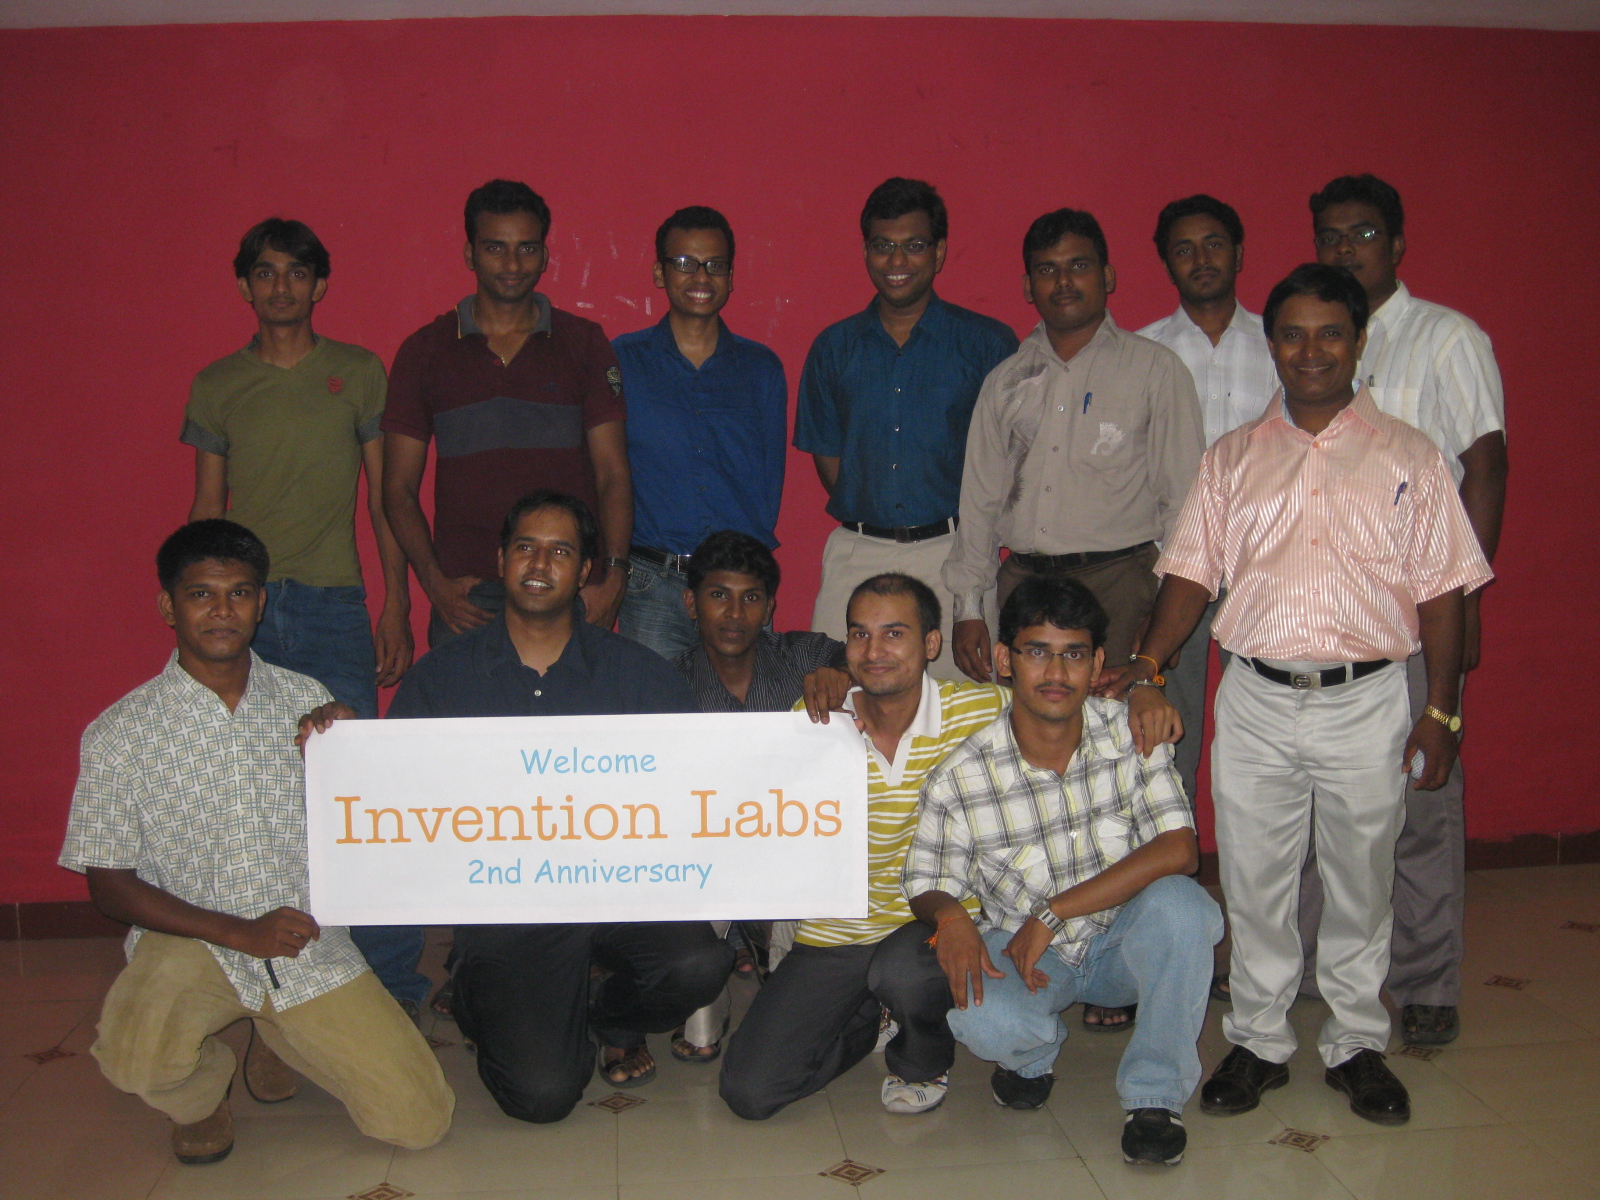
\includegraphics[scale=0.16]{images/Invention-Labs-Team.jpg} 
		\end{figure}
	\end{center}
\end{frame}

\begin{frame}
	\frametitle{About Inventors}
	\begin{itemize}
		\item Invention Labs is a startup based on Chennai and incubated at IIT Madras.
		\item Voted one of the hottest startups in India by Business Today in 2009.
		\item Invention Labs was founded by an alumni of IIT Madras.
	\end{itemize}
\end{frame}

\begin{frame}
	\frametitle{What is AVAZ?}
	\begin{itemize}
		\item AVAZ is an Augmentative and Alternative Communication (AAC) device for children with Cerebral Palsy.
		\item AVAZ is a portable speech synthesizer which can be controlled by gross motor movements of a child.
		\item This device helps speech-impaired children to become much more independent and free from their existing barriers.
		\item AVAZ is also portable, allowing the child to carry it around and even mount it on a wheelchair.
	\end{itemize}
\end{frame}

\begin{frame}
	\frametitle {Motivation of the device}
	\begin{itemize}
		\item Provide a \textcolor{red}{voice} to the non-verbal, allowing autistic children to communicate and express themselves
		\item For uplifting the autistic children.
		\item Enable speech-impaired children to communicate easily 
	\end{itemize}
\end{frame}

\section{timeline}
\begin{frame}
	\frametitle{Timeline of AVAZ}
	\tlcventry{2008}{2011}{AVAZ timeline}{}{}{}{}
	\tldatecventry[brown]{2008}{AVAZ }{company came up with idea}{}{}{}{}
	\tldatecventry[magenta]{2009}{AVAZ }{received 10 Lakh rupees grand from the Department of Scientific and Industrial Research}{Government of India}{}{}
	\tldatecventry[blue!70!black]{2010}{AVAZ}{beta version released}{}{}{}
	\tldatecventry[red]{2011}{AVAZ app version 1.0}{released on 18 May 2011}{}{}{}
\end{frame}

\section{commercialized}
\begin{frame}
	\frametitle {AVAZ is commercialized!}
	\begin{itemize}
		\item AVAZ device is \textcolor{red}{commercialized}.
		\item AVAZ app is available for iPad and Android.
		\item Invention Labs \textcolor{red}{earns} \$99 upon one app download.
	\end{itemize}
\end{frame}

\section{Opinion on IP}
\begin{frame}
	\frametitle {Intellectual property rights}
	\begin{itemize}
		\item Existing autism device costs around \$10,000 -- \$12,000. Where as AVAZ device costs only \$800. 
		\item As other autism device manufactures have \textcolor{red}{not} enforced IP, AVAZ became popular in the western countries and in India. 
		\item Decline to enforce the intellectual property rights by other device manufactures has strengthened AVAZ's market position.
	\end{itemize}
\end{frame}

\frame{
  	\vspace{2cm}
	\begin{center}
  		{\huge Thank you!}
	\end{center}
  	\vspace{1cm}
  	\begin{flushright}
        Seshagiri Prabhu \\
    	\structure{\footnotesize{seshagiriprabhu@gmail.com} \\ AM.EN.P2CSN12028 \\  \href{https://github.com/seshagiriprabhu/software-protection-lab}{Assignment repo}}
  	\end{flushright}
}

\end{document}